\chapter{Methodology}

\section{System Overview \& Architecture}
The proposed system implements a centralized, vision-based autonomous navigation architecture inspired by end-to-end learning paradigms. Unlike traditional autonomous robots that rely on onboard sensors (e.g., LIDAR, onboard cameras) and local processing, this framework offloads the computational workload to a remote workstation, utilizing a Bird’s Eye-view or overhead perspective. The architectural data flow, detailing the transition from physical sensing to robot actuation, is illustrated in Figure 3.1.

\begin{figure}[!ht]
    \centering
    {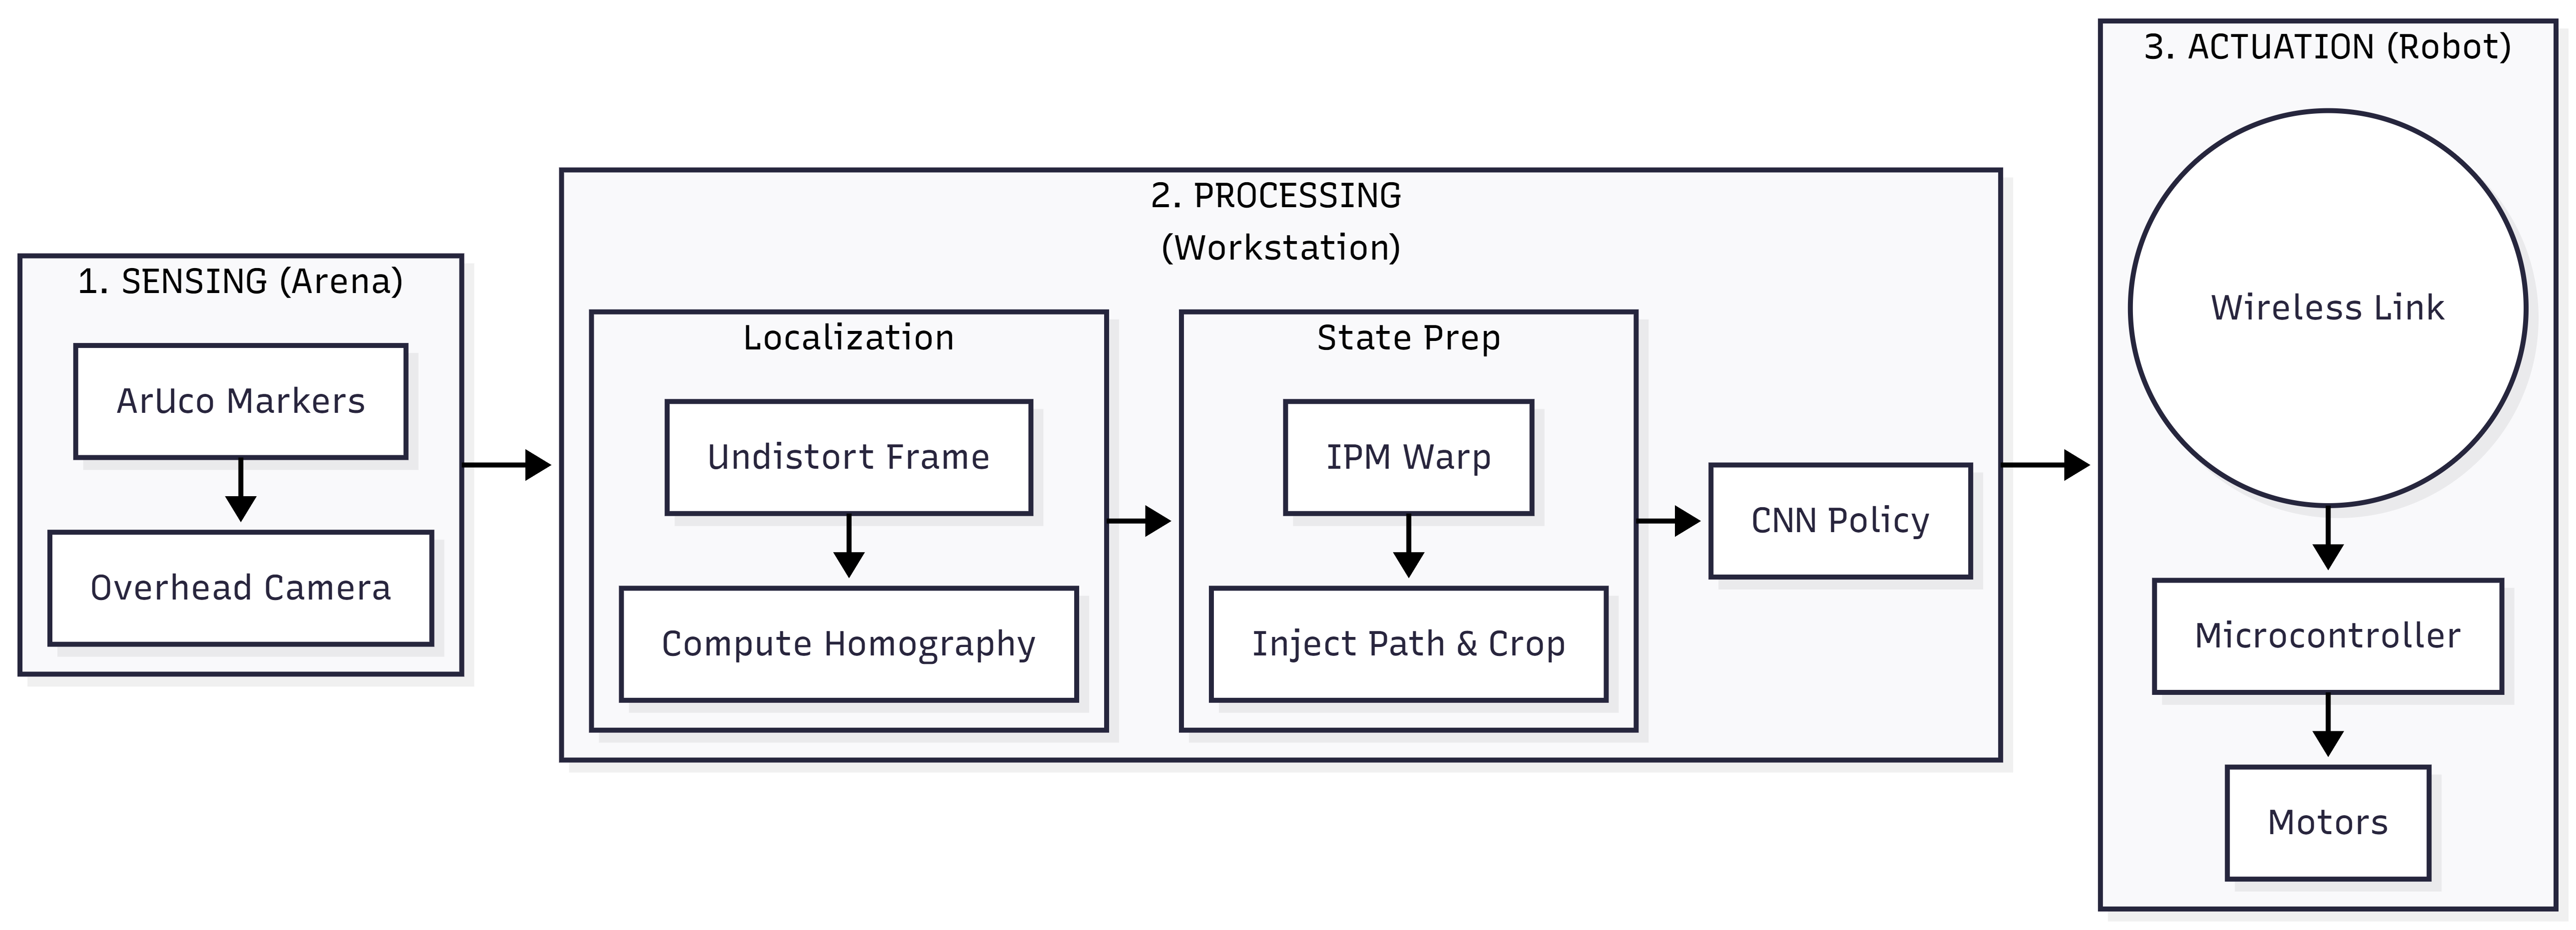
\includegraphics[width=1.0\textwidth]{images/figure3_1.png}}\qquad
    \caption[Short Caption]{System Architecture.}        
    \label{fig:3.1}
\end{figure}


As depicted in Figure~\ref{fig:3.1}, the system architecture is divided into three functional subsystems: sensing, processing, and actuation. Together, these components form a closed-loop control pipeline for autonomous navigation.

\begin{itemize}
    \item \textbf{Sensing Subsystem (Arena):}  
    Located in the physical environment, this block consists of an overhead camera and fixed ArUco markers. The camera captures the entire operational arena and provides the raw visual input used by the system. The ArUco markers act as reference points for geometric correction and spatial alignment.

    \item \textbf{Processing Subsystem (Workstation):}  
    This block contains the core intelligence of the system and executes a two-stage processing pipeline:
    \begin{itemize}
        \item \textbf{Localization and State Preparation:}  
        The system detects ArUco markers to compute a homography matrix, which warps the angled camera feed into a standardized top-down bird’s-eye view using inverse perspective mapping (IPM). The transformed image is cropped and augmented with the target navigation path to form the system state.
        
        \item \textbf{CNN-Based Policy Inference:}  
        The pre-processed visual state is fed directly into a convolutional neural network (CNN), which serves as an end-to-end behavioral policy mapping visual observations directly to low-level motor control commands.
    \end{itemize}

    \item \textbf{Actuation Subsystem (Robot):}  
    The inferred control commands, including steering and throttle signals, are transmitted wirelessly via Wi-Fi or Bluetooth to the mobile robot. The robot’s onboard microcontroller receives these commands and drives the motors, completing the closed-loop control cycle.
\end{itemize}

\section{Hardware Setup}

\subsection{Robot Platform}
The mobile agent utilized in this study is a custom-built differential drive robot designed for low-latency execution of remote commands. The platform is intentionally minimized to function as a "remote-controlled" agent, removing the need for heavy onboard computation.

    \begin{itemize}
        \item \textbf{Chassis and Drivetrain:} 
        The robot is built on a standard 2-wheel drive (2WD) chassis with a caster wheel for stability. It utilizes two DC gear motors configured for Differential Drive kinematics, allowing for zero-radius turning and precise heading adjustments.
        \item \textbf{Microcontroller:}
         The robot is equipped with a low-cost microcontroller (e.g., Raspberry Pi 4 or Nvidia Jetson Nano) acting as a communication bridge. Its sole function is to receive data packets from the central workstation and convert them into Pulse Width Modulation (PWM) signals.
         \item \textbf{Motor Driver:}
          An H-Bridge motor driver (e.g., L298N or TB6612FNG) is used to interface the microcontroller with the DC motors, providing the necessary current amplification and direction control.
          \item \textbf{Power Supply:}
           The system is powered by a Lithium-Ion battery pack (e.g., 2S or 3S 18650 configuration), regulated to provide stable voltage to the microcontroller and raw power to the motor driver.
    \end{itemize}

\subsection{Environment Setup}
The experimental environment is a controlled, structured arena designed to implement computer vision processing. A single high-definition RGB webcam (Logitech BRIO) is mounted at a fixed height above the area. The camera is positioned at an angle to cover the entire operational area. While the camera is angled, the software pipeline corrects this perspective distortion mathematically. The arena consists of a flat, non-reflective surface (to minimize glare and specular highlights that could confuse the CNN). The boundaries of the Region of Interest (ROI) are physically defined by four ArUco markers fixed at the corners. These markers serve as the static reference anchors for the system's homography calibration. All image processing, neural network training, and real-time inference are performed on a dedicated laptop or desktop computer equipped with a GPU. This workstation runs the Python-based control software, processes the camera feed via USB, and broadcasts control commands to the robot over the local wireless network.




\section{Camera and System Calibration}
To ensure that the visual input fed into the neural network accurately represents the physical world, the system undergoes a rigorous calibration process. This separates the intrinsic properties of the camera (lens distortion) from the geometric relationship between the camera and the arena (homography).
The goal of intrinsic calibration is to estimate the camera matrix K (focal lengths and principal point) and distortion coefficients so that the image pixels and rays can be mapped in 3-D. Firstly, we introduce the pinhole model \citep{Hartley2004}, where a scene view is formed by projecting 3D points into the image plane using a perspective transformation. 

\begin{equation}
    s \begin{bmatrix} u \\ v \\ 1 \end{bmatrix} = K \begin{bmatrix} X \\ Y \\ Z \\ 1 \end{bmatrix}
\end{equation}

\noindent where:
\begin{itemize}
    \item $(X, Y, Z)$ are the coordinates of a 3D point in the world coordinate space.
    \item $(u, v)$ are the coordinates of the projection point in pixels.
    \item $s$ is a scaling factor.
\end{itemize}

However, camera lenses introduce lens distortion where lines may appear deformed. Mostly, these distortions are classified as radial distortion and slight tangential distortion (Brown, 1966). Webcam cameras, particularly the wide-angle lens on the Logitech BRIO used in this study—introduce radial and tangential distortion. To address this, the pinhole model above is augmented with a vector of distortion coefficients. These distortions are addressed using the following distortion model:

\noindent Radial Distortion:
\begin{equation}
    x_{corrected} = x(1 +k_1r^2 + k_2r^4 + k_3r^6)
    \label{radialDistortX}
\end{equation}
\begin{equation}
    y_{corrected} = y(1 +k_1r^2 + k_2r^4 + k_3r^6)
    \label{radialDistortY}
\end{equation}

\noindent Tangential Distortion
\begin{equation}
    x_{corrected} = x + [2p_1xy + p_2(r^2 + 2x^2]
\end{equation}
\begin{equation}
    y_{corrected} = y + [p_1(r^2 + 2y^2) + 2p_2xy]
\end{equation}

\noindent where:
\begin{itemize}
    \item \(k_1, k_2, k_3\) are radial coefficients,
    \item \(p_1, p_2\) are tangential coefficients and
    \item \(r^2 = x^2 + y^2\)
\end{itemize}

In OpenCV \citep{Bradski2000OpenCV}, these are grouped into a distortion vector that typically contains radial terms and tangential terms. All distortion coefficients are treated as intrinsic parameters of the camera. And once these coefficients are estimated, they remain valid for that camera regardless of the scene and can be reused at varying image resolutions, with only the focal length and principal point scaled if the resolution changes. 

\noindent\textbf{Calibration Procedure}

Intrinsic parameters are obtained using a standard checkerboard calibration method based on \cite{Zhang2000CameraCalibration}. We use the function \verb |calibrateCamera| then a planar checkerboard with known square dimensions is captured from multiple viewpoints. The inner corners are detected in each image, creating a set of 2D pixel observations corresponding to known 3D grid coordinates. The function uses the Levenberg-Marquardt optimization algorithm \citep{Levenberg1944LeastSquares} to minimize the reprojection error, defined as the sum of squared distances between the observed feature points (detected corners) and the projected object points (computed using current estimates of K and distortion coefficients). This process outputs the optimal intrinsic matrix and distortion vector, which are then stored for real-time image correction.

\section{Perception and Localization Module}
To enable autonomous navigation, the system requires a robust method to define the valid operational area and pre-process visual data for the neural network. This is achieved using fiducial markers to define the Region of Interest (ROI) and applying a projective transformation to normalize the visual input. This perception module operates in two distinct phases:

\begin{itemize}
    \item Initialization Phase: A one-time setup process that detects static arena boundaries and computes the coordinate mapping (from Section 3.3.2).
    \item Runtime Phase: A continuous loop that corrects and warps visual data in real-time for the control policy.
\end{itemize}

\subsection{ArUco Marker Detection}
\label{sec:3.4.1}
The localization pipeline begins with the detection of ArUco markers (Garrido-Jurado et al., 2014),  to define the Area of Interest (AOI). We utilize the \verb|DICT_4X4_50 |dictionary (4x4 bit grid, 50 unique IDs), which offers a balance between decoding speed and false-positive rejection.

\noindent\textbf{Marker Configuration and Corner Assignment}

To resolve the ambiguity of the arena’s orientation and prevent the coordinate system from mirroring or rotating if the camera placement changes, specific unique IDs are assigned to the four physical corners of the operational area. This fixed assignment acts as a ground truth for the homography estimation. The configuration is explicitly defined as follows:
\begin{enumerate}
    \item Top-Left (TL): Marker ID 0
    \item Top-Right (TR): Marker ID 1
    \item Bottom-Right (BR): Marker ID 2
    \item Bottom-Left (BL): Marker ID 3
\end{enumerate}

During the initialization part, the system does not simply accept any four detected markers. It filters the detected markers to find these specific IDs. Once these markers are found, they are sorted into a strictly ordered list \verb|[TL, TR, BR, BL]|, which is then used to get the homography matrix discussed in the later section.

Essentially, detection is performed on the undistorted frame. If detection were performed on the raw frame, the resulting Homography matrix would incorporate lens distortion, leading to a warped coordinate system where straight trajectories appear curved. By undistorting first, we ensure that the detected marker corners correspond to linear projective geometry.

\noindent The detection pipeline proceeds as follows:
\begin{enumerate}
    \item Preprocessing: The input RGB frame is converted to grayscale to simplify intensity analysis.
    \item Candidate Extraction: Adaptive thresholding is applied to segment black borders. Contours are extracted from the thresholded image and filtered based on convexity and square geometry.
    \item Bit Extraction and Decoding: The inner region of candidate squares is divided into a grid. The pixel intensity of each cell is analyzed to form a binary matrix.
    \item Corner Refinement: To ensure high-precision localization, corner positions are refined to sub-pixel accuracy using the \verb|cornerSubPix| algorithm
\end{enumerate}

The output is a set of four ordered corner coordinates from the undistorted image. It should be noted that these markers are not attached to the robot, they serve only to anchor the global coordinate system of the arena for the homography calculation.

\subsection{Planar Homography Estimation}
\label{sec:3.4.2}
Unlike the usual 3D pose estimation, this study limits the robot’s movement to a 2D planar surface. Additionally, the geometric relationship between the camera’s image plane and the physical world plane is modeled as a Planar Homography \citep{Hartley2003MultipleViewGeometry}. A homography is an invertible projective transformation that maps points from one plane (image pixel plane) \(p = [u,v,1]^T\) and a world coordinate \(P_w = [x,y,1]^T\) is given by:

\begin{equation}
    s[u,v,1] = H [u,v,1]
\end{equation}

where \(H\) is a \(3 \times 3\) matrix with 8 degrees of freedom

To compute H, we utilize the set of four physical points obtained from the ArUco markers (Section \ref{sec:3.4.1}), placed at the corners of the area of interest. Theoretically, this is solved using the Direct Linear Transformation (DLT) algorithm \citep{AbdelAziz2015DLT}. This algorithm rewrites the correspondence equation \(sx' = Hx\)  into a system of linear equations of the form \(Ah = 0\), where \(h\) is a vector containing the entries of \(H\). 

Since exactly four corresponding point pairs are established using the sorted ArUco IDs, we utilize the \verb|getPerspectiveTransform| function in OpenCV. This function computes the \(3 \times 3\) transformation matrix analytically. This method relies on the ground-truth correspondence provided by the unique marker IDs, which establishes a deterministic and geometrically accurate mapping.

\noindent \textbf{Perspective Warping (Runtime Application)
}

During runtime, the raw camera feed, which contains the arena viewed from an angle as well as irrelevant background noise is transformed using Perspective Warp. Leveraging the pre-computed \(H\), we map the entire input frame to a standardized top-down view. This is done through the use of the \verb|warpPerspective| function from OpenCV.

\begin{equation}
    Img_{world} = warpPerspective(Img_{raw}, H)
\end{equation}

This transformation creates a rectified "Bird's Eye View" image where the four corner markers perfectly align with the corners of the image frame. This ensures that the Convolutional Neural Network (CNN) receives an input that is geometrically constant regardless of slight shifts in camera placement or angle. This warped image serves as the direct input to the End-to-End control network, allowing the model to infer the robot's position and orientation from the visual features of the robot relative to the arena floor.

\subsection{Grid Map and Obstacle Representation}

To enable path planning and state observation, the continuous world coordinates are discretized into a Grid Map (Occupancy Grid). To define the grid, the area of interest is divided into \(N \times M\) matrix of cells, where each cell represents a fixed physical area defined by the resolution \(\delta\) (meters per cell). The mapping from World Coordinates \((x, y)\) to Grid Indices \((r, c)\) is defined as:

\begin{equation}
    c = |\frac{{x-x_{min}}}{\delta}|, r = |\frac{y-y_{min}}{\delta}|
\end{equation}

\noindent where:
\begin{itemize}
    \item \((x, y)\) are the metric coordinates of the point on the arena floor.
    \item \((x_{min}, y_{min})\) is the origin of the area in world coordinates.
    \item \(\delta\) is the resolution. 
\end{itemize}

We designated cells inside the area of interest between two states, free and obstacle. A cell in the grid matrix \(\bold{B}\) is assigned a binary value, a cell \(G[r,c]\) will be set to zero to denote an empty or clear space, which is safe for robot traversal. On the other hand, a cell will be set to one to denote an obstacle or restricted area.

This binary grid serves as the logical model of the environment. However, the neural network operates on the high-resolution visual equivalent, which is the warped image derived in Section \ref{sec:3.4.2}. Because the homography transformation rectifies the camera view, the input image tensor shares this exact Euclidean grid structure. This ensures spatial consistency, meaning that a movement of pixels in the input tensor always corresponds to a fixed physical distance in the real world, regardless of the camera's original perspective.


\section{Convolutional Neural Network}

This section details the implementation of the deep learning pipeline, translating the theoretical framework of Behavioral Cloning and CNNs (discussed in Section 2.7) into a functional navigation system. The pipeline is divided into model architecture design, data preprocessing, acquisition, training, and final deployment.
\subsection{Model Architecture}

The study employs a custom convolutional neural network (CNN) architecture designed for regression tasks. Unlike classification networks that output probability distributions over discrete categories, the proposed network predicts continuous control values. The architecture follows an encoder--decoder style flow adapted for control applications, beginning with an input layer that accepts preprocessed image tensors, with dimensions defined in Section~3.6.2.

The core processing is performed by a convolutional feature extractor composed of three sequential convolutional layers that extract spatial features from the homography-transformed overhead view. The first two layers employ smaller kernel sizes (e.g., $3 \times 3$) to capture fine-grained spatial details, such as the robot's orientation relative to the navigation path. The third convolutional layer uses a larger kernel size to capture higher-level spatial hierarchies. Each convolutional layer applies a Rectified Linear Unit (ReLU) activation function, defined as $f(x) = \max(0, x)$, to introduce non-linearity.

Following feature extraction, a flattening operation converts the multidimensional feature maps into a one-dimensional vector, preparing the data for high-level reasoning.

\begin{figure}[!ht]
    \centering
    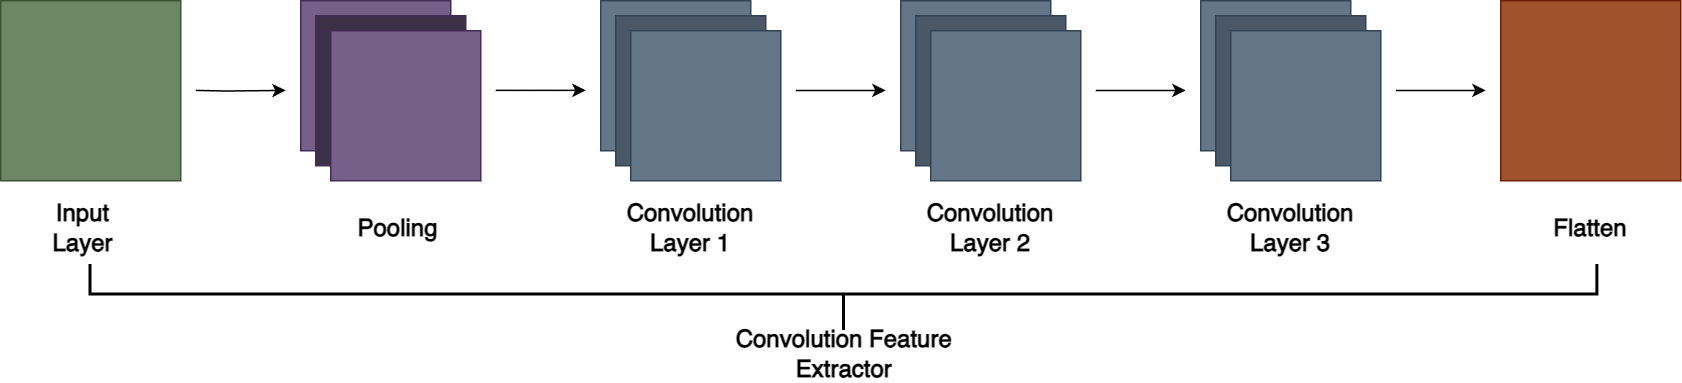
\includegraphics[width=1\textwidth]{images/figureCNN.png}
    \caption{Feature Extraction Block: Input, Convolutional Layers, and Flattening}
    \label{fig:CNN}
\end{figure}

Once flattened, the data is passed through a series of fully connected (dense) layers. Two dense layers are used to interpret the extracted spatial features, with the final hidden layer employing a reduced number of neurons to serve as a decision-making bottleneck. The network concludes with an output layer consisting of two neurons with a linear activation function. These output neurons correspond directly to the vehicle's actuation signals: $y_1$, representing the steering command (normalized steering angle or differential ratio), and $y_2$, representing the throttle or velocity command (normalized pulse-width modulation (PWM) duty cycle).

\begin{figure}[!ht]
    \centering
    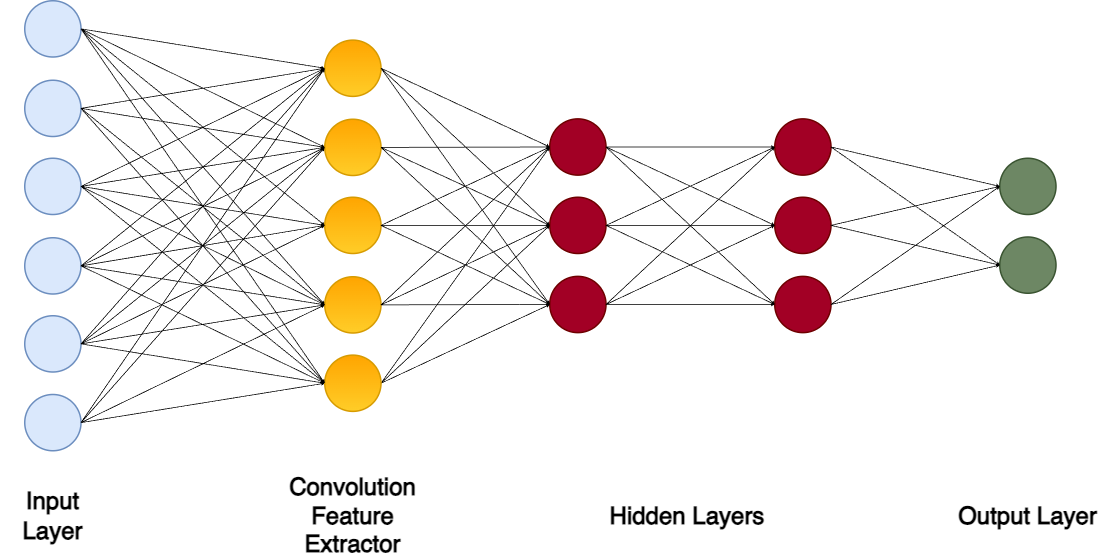
\includegraphics[width=1\linewidth]{images/figure_neural_net.png}
    \caption{Neural Network Diagram: Fully Connected Layers and Actuation Outputs}
    \label{fig:Neural_net}
\end{figure}

\subsection{Input Preprocessing and State Representation}
To ensure the network learns the vehicle's kinematics rather than environmental noise, the raw visual data undergoes rigorous preprocessing based on the homography principles established in Section 2.7.1.

\begin{figure}[!ht]
        \centering
        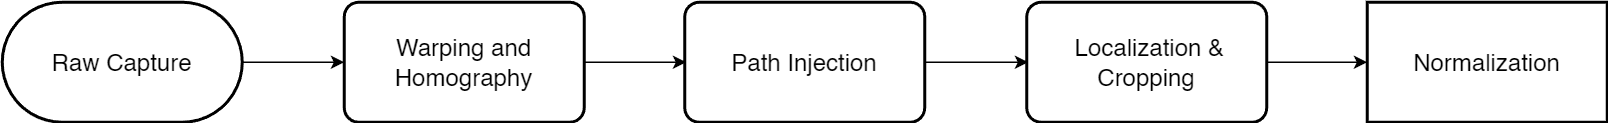
\includegraphics[width=0.9\linewidth]{images/figure_preprocessing.png}
        \caption{The image preprocessing pipeline converting raw camera input into a state representation for the CNN}
        \label{fig:preprocess}
    \end{figure}

\begin{itemize}
    \item \textbf{Homography Transformation:} The raw feed from the overhead camera is warped using the homography matrix $H$, computed via the Direct Linear Transformation (DLT) algorithm. This operation converts the perspective view into a top-down, metric-accurate orthographic representation of the arena.

    \item \textbf{State Augmentation (Path Injection):} To provide the robot with a navigation objective, the target coverage path is digitally rendered onto the transformed image. This results in a composite state representation that encodes both the robot's current pose and the desired trajectory.

    \item \textbf{Region of Interest (ROI) Cropping:} To reduce computational complexity, a fixed-size image crop centered on the robot's coordinates (e.g., $100 \times 100$ pixels) is extracted. This focuses the network on local path-following behavior rather than the full arena context.

    \item \textbf{Normalization:} Pixel intensity values, originally in the integer range $[0,255]$, are normalized to a floating-point range of $[0,1]$ (or $[-1,1]$) to promote numerical stability and faster convergence during gradient-based optimization.
\end{itemize}
\subsection{Data Acquisition and Model Training Pipeline}
Following the Behavioral Cloning paradigm (Section 2.7.3), a dataset will be constructed to capture expert human driving behavior. This study will utilize an Imitation Learning approach, specifically Behavioral Cloning, where the goal is to learn a control policy that mimics expert human driving behavior. The process is divided into two phases: dataset construction and supervised network training. The complete workflow, from the initial capture of human demonstrations to the final optimization of the neural network, is illustrated in \ref{fig:acquisition_training}
\begin{figure}[!ht]
    \centering
    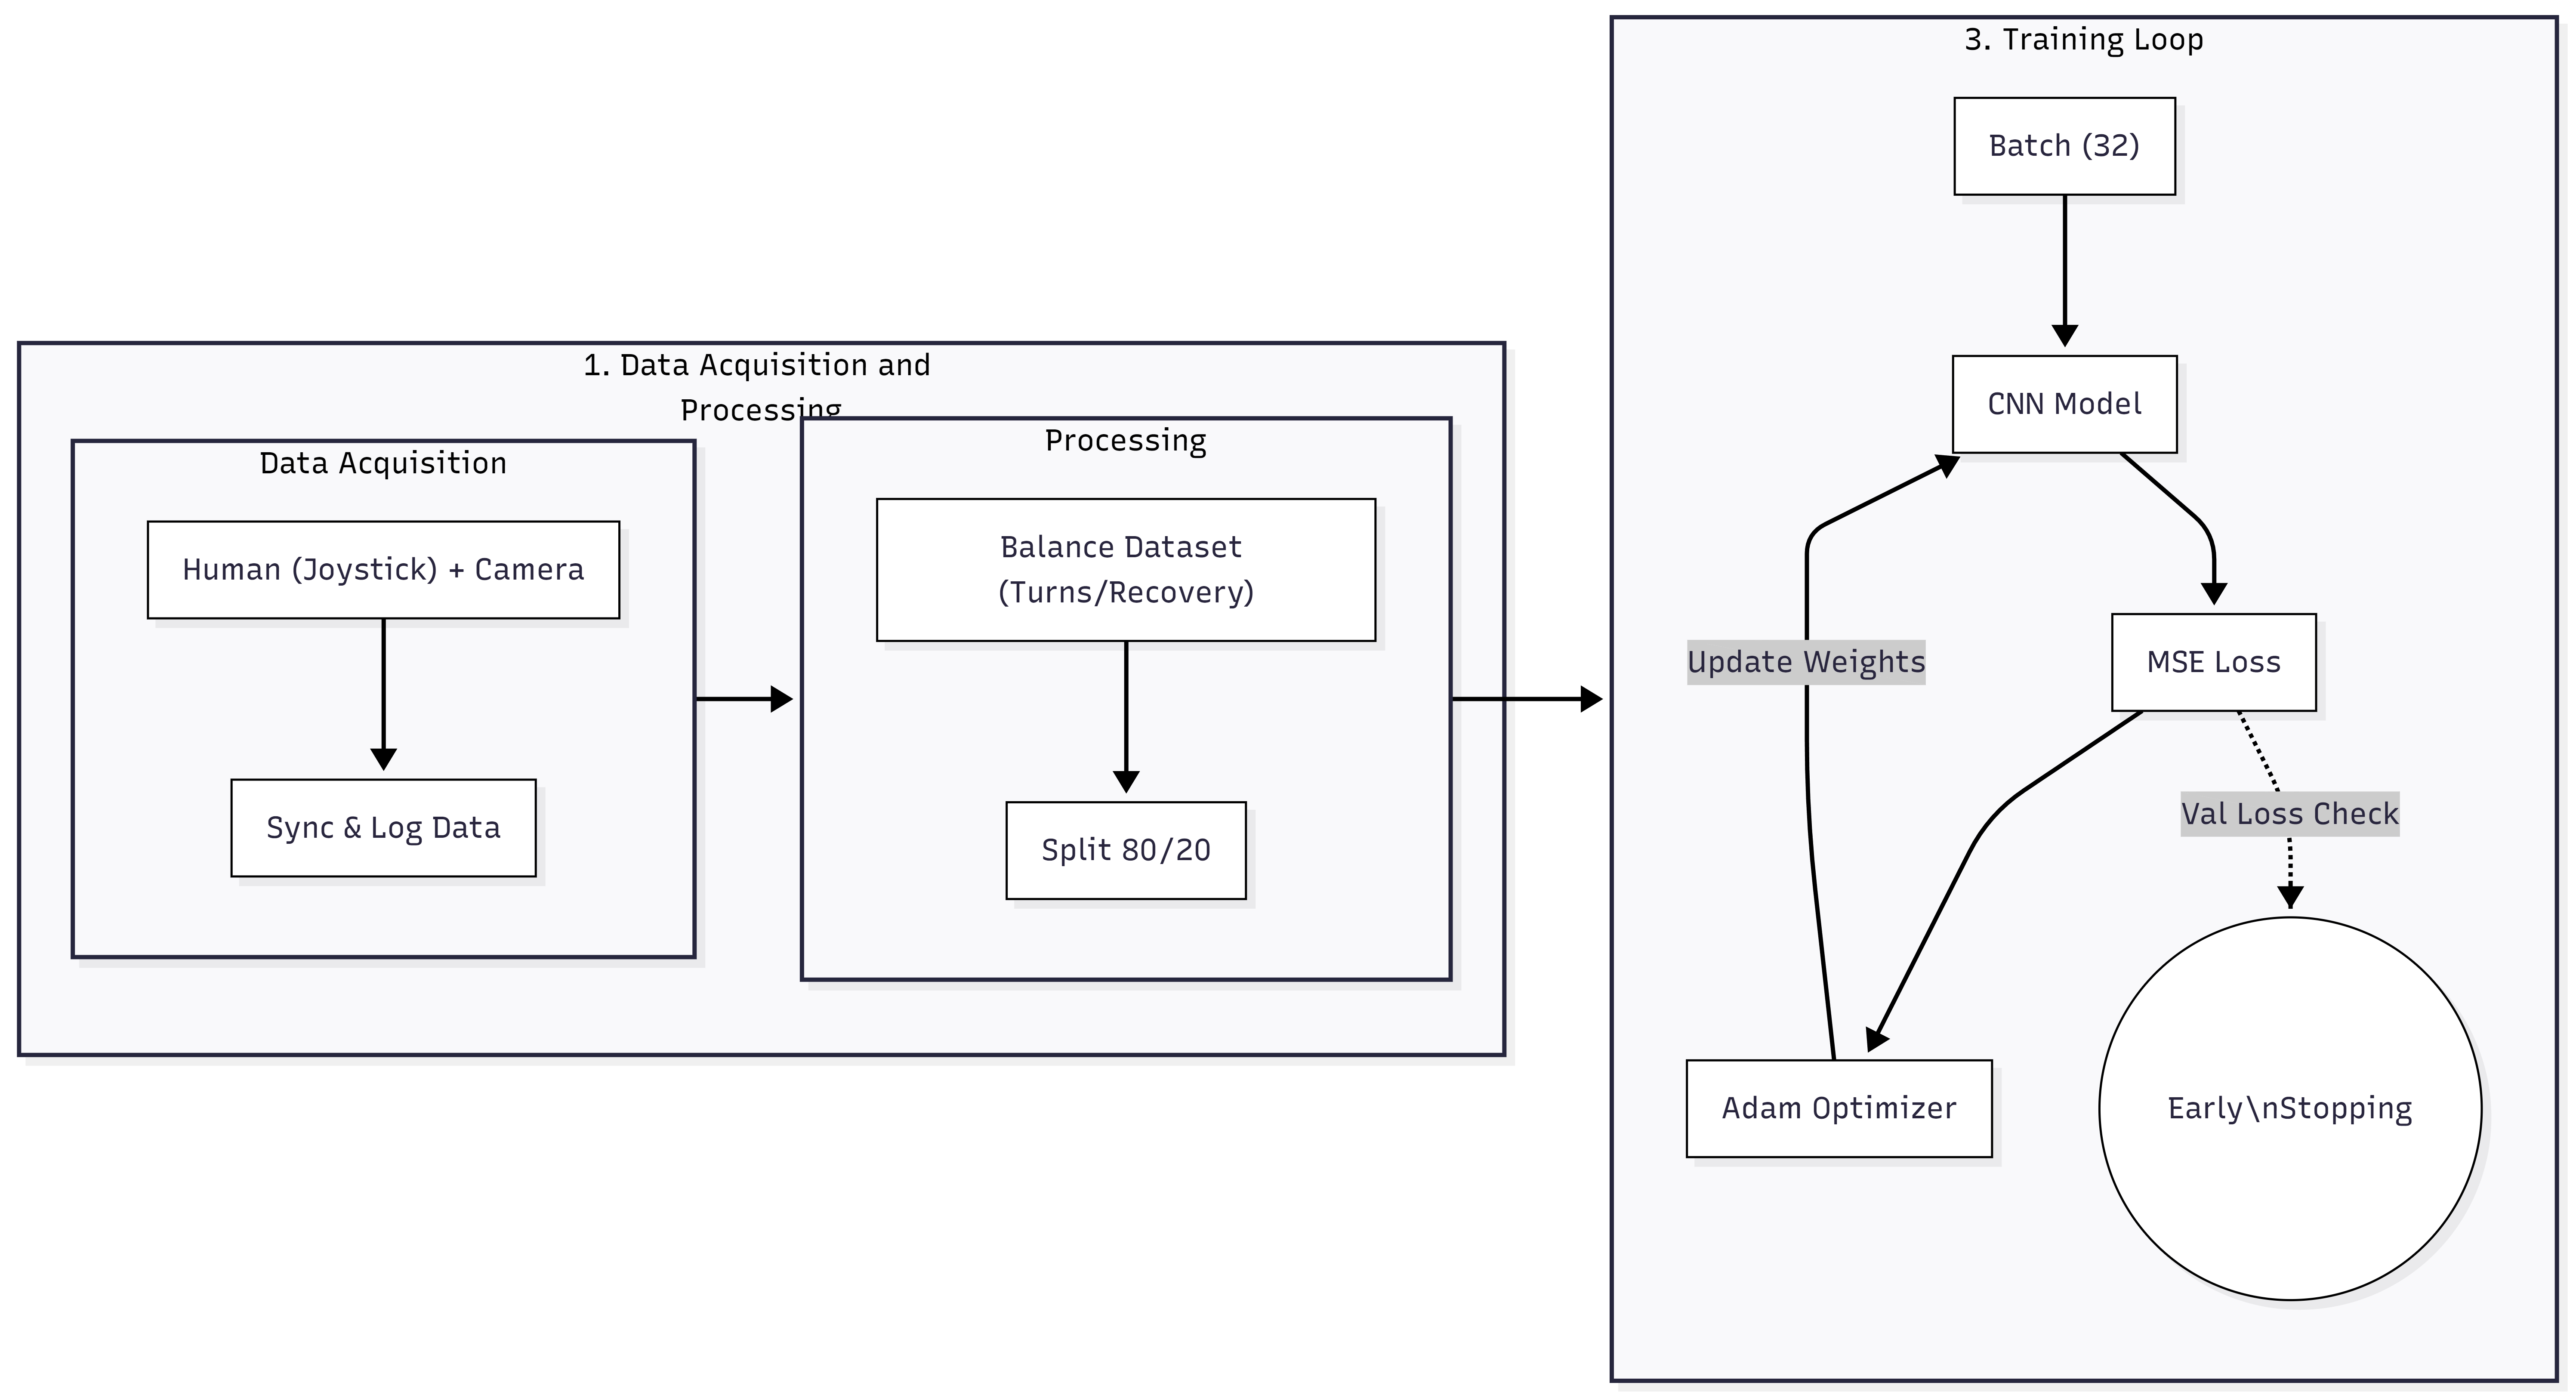
\includegraphics[width=0.7\linewidth]{images/figure_acquisition_training.png}
    \caption{Data Acquisition and Training Pipeline}
    \label{fig:acquisition_training}
\end{figure}

\subsection*{Phase 1: Data Acquisition and Processing}

As shown in the first stage of Figure~3.5, the dataset
\[
\mathcal{D} = \{(s_i, a_i)\}_{i=1}^{N}
\]
is generated by manually controlling the robot using a joystick or gamepad. During these runs, the overhead camera system executes the preprocessing pipeline in real time. A specialized data logger script synchronizes the visual input (state $s_i$) with the human's control inputs (action $a_i$).

\begin{itemize}
    \item \textbf{State ($s_i$):} The preprocessed, cropped image frame.
    \item \textbf{Action ($a_i$):} The control tuple recorded from the joystick.
\end{itemize}

To ensure the model generalizes well and avoids \emph{straight-line bias}, the dataset is balanced to include a diverse distribution of driving scenarios. This explicitly includes straight segments, left and right turns, and recovery maneuvers—instances where the robot is intentionally driven off-path and then corrected—teaching the network how to return to the track center.

\subsection*{Phase 2: Training Configuration}

The network is trained as a regression task using the collected dataset. As depicted in the Training Loop of Figure~3.5, the optimization objective is to minimize the Mean Squared Error (MSE), defined as the Euclidean distance between the predicted control vector and the human’s actual control vector:

\[
\mathcal{L} = \frac{1}{N} \sum_{i=1}^{N}
\left\| y^{(i)}_{\text{pred}} - y^{(i)}_{\text{true}} \right\|^2
\]

The Adam optimizer is selected for its adaptive learning rate capabilities, ensuring stable convergence given the non-convex nature of the loss landscape. An 80:20 dataset split is employed, with 80\% used for training and 20\% for validation. A batch size of 32 is used, and training proceeds until the validation loss plateaus, at which point Early Stopping is applied to prevent overfitting.
\subsection{Deployment and Inference}
\label{sec:deployment_inference}

The trained model is exported and optimized for the target hardware. The deployment process operates in a continuous control loop.

\begin{enumerate}
    \item \textbf{Model Serialization:} The trained network architecture and weights are saved in a portable format (e.g., \texttt{.h5} or \texttt{.tflite}).

    \item \textbf{Inference Loop:} The deployment script runs on the central processing unit (CPU) or the robot’s onboard computer in a continuous loop:
    \begin{enumerate}[\alph*.]
        \item Capture and warp the overhead camera image using the homography transformation.
        \item Preprocess the image and extract the Region of Interest (ROI).
        \item Feed the processed sensor input into the Convolutional Neural Network (CNN).
        \item The CNN outputs raw regression values corresponding to control commands (e.g., steering = 0.3, throttle = 0.8).
        \item The predicted values are scaled to the appropriate PWM range (0--255) and transmitted directly to the motor drivers via GPIO, bypassing any PID or additional error-correction logic.
    \end{enumerate}
\end{enumerate}
% \begin{figure}[!ht]
%     \centering
%     \subbottom[Goku]{
\includegraphics[width=0.3\textwidth]{test_image_goku}}\qquad
%     \subbottom[More Goku]{
\includegraphics[width=0.3\textwidth]{test_image_goku}}%
%     \caption[Short Caption]{The same super saiyan. Two times.}        
%     \label{fig:test2}
% \end{figure}

% Two figures shown side by side are shown in Figure~\ref{fig:test2}.

% \begin{table*}\centering
% \ra{1.3}
% \begin{tabular}{@{}rrrrcrrr@{}}\toprule
% & \multicolumn{3}{c}{$w = 8$} & \phantom{abc}& \multicolumn{3}{c}{$w = 16$} \\
% \cmidrule{2-4} \cmidrule{6-8} 
% & $t=0$ & $t=1$ & $t=2$ && $t=0$ & $t=1$ & $t=2$\\ \midrule
% $dir=1$\\
% $c$ & 0.0790 & 0.1692 & 0.2945 && 0.3670 & 0.7187 & 3.1815\\
% $c$ & -0.8651& 50.0476& 5.9384&& -9.0714& 297.0923& 46.2143\\
% $c$ & 124.2756& -50.9612& -14.2721&& 128.2265& -630.5455& -381.0930\\
% $dir=0$\\
% $c$ & 0.0357& 1.2473& 0.2119&& 0.3593& -0.2755& 2.1764\\
% $c$ & -17.9048& -37.1111& 8.8591&& -30.7381& -9.5952& -3.0000\\
% $c$ & 105.5518& 232.1160& -94.7351&& 100.2497& 141.2778& -259.7326\\
% \bottomrule
% \end{tabular}
% \caption{A Beautiful and Complex Table}\label{tab:sometable}
% \end{table*}
\section{Software Architecture}

This section details the software framework governing the autonomous vehicle. The system is designed as a modular, monolithic application primarily implemented in Python, leveraging libraries such as OpenCV for computer vision and TensorFlow/PyTorch for deep learning inference. The architecture prioritizes low latency to ensure the end-to-end control loop maintains a sufficient frequency for stable navigation.

\subsection{Module Integration}
\label{sec:module_integration}

The software is organized into four distinct functional modules. This modular design ensures separation of concerns, allowing for easier debugging and independent testing of subsystems (e.g., testing image warping without running the motors). The core modules are defined as follows:

\begin{enumerate}
    \item \textbf{Perception Interface (\textit{CameraStream}):}
    \begin{itemize}
        \item Responsible for interfacing with the hardware camera driver.
        \item Manages the frame buffer to ensure the processing pipeline always retrieves the most recent frame, discarding stale data to minimize input lag.
    \end{itemize}

    \item \textbf{State Estimator (\textit{Preprocessor}):}
    \begin{itemize}
        \item Encapsulates the geometric logic described in Section~3.4.
        \item Contains the pre-calculated homography matrix $H$ and performs the perspective warp and ROI cropping.
        \item Handles the normalization of pixel values before passing sensor data to the neural network.
    \end{itemize}

    \item \textbf{Inference Engine (\textit{PilotModel}):}
    \begin{itemize}
        \item Loads the pre-trained CNN model weights into memory during initialization.
        \item Provides a \texttt{predict()} method that accepts the processed image tensor and returns the raw steering and throttle outputs.
        \item Is optimized to run on the specific hardware accelerator (e.g., GPU or Neural Processing Unit), if available.
    \end{itemize}

    \item \textbf{Actuation Interface (\textit{MotorDriver}):}
    \begin{itemize}
        \item Abstracts the low-level GPIO (General Purpose Input/Output) commands.
        \item Converts the normalized CNN output (e.g., $[-1,1]$ or $[0,1]$) into hardware-specific PWM duty cycles (e.g., 0--255 or 0--65535).
        \item Includes safety stops, ensuring the motors default to zero velocity if the software is interrupted.
    \end{itemize}
\end{enumerate}
\begin{algorithm}[H]
\caption{Homography Estimation and Perspective Warping}
\label{alg:homography_warping}
\begin{algorithmic}[1]

\Function{InitializeAndWarp}{$raw\_frame, camera\_matrix, dist\_coeffs, arena\_dims$}
\State \textbf{Input:}
\State \hspace{1em} $raw\_frame$ — Raw RGB image from the camera
\State \hspace{1em} $camera\_matrix (K), dist\_coeffs (D)$ — Intrinsic calibration parameters
\State \hspace{1em} $arena\_dims$ — Target width and height of bird's-eye view
\State \textbf{Output:} $warped\_frame, homography\_matrix$

\Statex
\State \textbf{// Phase 1: Undistortion}
\State $undistorted\_frame \gets \textsc{Undistort}(raw\_frame, K, D)$
\State $gray\_frame \gets \textsc{ConvertToGray}(undistorted\_frame)$

\Statex
\State \textbf{// Phase 2: Marker Detection}
\State $dictionary \gets \textsc{GetDictionary}(\texttt{DICT\_4X4\_50})$
\State $(corners, ids) \gets \textsc{DetectMarkers}(gray\_frame, dictionary)$

\Statex
\State \textbf{// Phase 3: ID-Based Sorting (Ground Truth Assignment)}
\State \textbf{// Marker IDs: 0=TL, 1=TR, 2=BR, 3=BL}
\State $expected\_ids \gets \{0,1,2,3\}$

\If{$|ids| < 4$ \textbf{or} $expected\_ids \not\subseteq ids$}
    \State \Return \textbf{Error} ``Markers 0--3 not found''
\EndIf

\State $src\_points \gets$ empty list of size $4$

\For{$i \gets 1$ to $|ids|$}
    \If{$ids[i] = 0$}
        \State $src\_points[0] \gets corners[i]$ \Comment{Top-Left}
    \ElsIf{$ids[i] = 1$}
        \State $src\_points[1] \gets corners[i]$ \Comment{Top-Right}
    \ElsIf{$ids[i] = 2$}
        \State $src\_points[2] \gets corners[i]$ \Comment{Bottom-Right}
    \ElsIf{$ids[i] = 3$}
        \State $src\_points[3] \gets corners[i]$ \Comment{Bottom-Left}
    \EndIf
\EndFor

\Statex
\State \textbf{// Phase 4: Homography Calculation}
\State $dst\_points \gets \{(0,0), (W,0), (W,H), (0,H)\}$
\State $homography\_matrix \gets \textsc{GetPerspectiveTransform}(src\_points, dst\_points)$

\Statex
\State \textbf{// Phase 5: Perspective Warping}
\State $warped\_frame \gets \textsc{WarpPerspective}(undistorted\_frame, homography\_matrix, arena\_dims)$

\State \Return $warped\_frame, homography\_matrix$
\EndFunction

\end{algorithmic}
\end{algorithm}

\begin{algorithm}[H]
\caption{Navigation Agent: Neural Network Inference}
\label{alg:inference_logic}
\begin{algorithmic}[1]

\Function{ComputeControlVector}{$warped\_frame, cnn\_model$}
    \State \textbf{Input:} Top-down image and pre-trained CNN model
    \State \textbf{Output:} Steering angle and throttle commands

    \Statex
    \State \textbf{// Step 1: Pre-processing}
    \State $input \gets \textsc{Resize}(warped\_frame, 66 \times 200)$
    \State $input \gets \textsc{NormalizePixelValues}(input)$ \Comment{Scale to range [0, 1]}

    \Statex
    \State \textbf{// Step 2: Deep Learning Inference}
    \State $(raw\_steer, raw\_throttle) \gets \textsc{ModelPredict}(cnn\_model, input)$

    \Statex
    \State \textbf{// Step 3: Safety Saturation}
    \State \Comment{Clip outputs to ensure values are within hardware limits}
    \State $steering \gets \textsc{Clip}(raw\_steer, -1.0, 1.0)$
    \State $throttle \gets \textsc{Clip}(raw\_throttle, 0.0, 1.0)$

    \State \Return $steering, throttle$
\EndFunction

\end{algorithmic}
\end{algorithm}

\begin{algorithm}[H]
\caption{Actuation: Hardware Control Interface}
\label{alg:actuation_logic}
\begin{algorithmic}[1]

\Function{DriveRobot}{$steering, throttle$}
    \State \textbf{Input:} Normalized control commands from Neural Network
    \State \textbf{Output:} Physical electrical signals to motors

    \Statex
    \State \textbf{// Step 1: Safety Check}
    \If{Watchdog Timer Expired}
        \State \textsc{TriggerEmergencyStop}()
        \State \Return
    \EndIf

    \Statex
    \State \textbf{// Step 2: Signal Conversion}
    \State \Comment{Convert normalized values to Pulse Width Modulation (PWM)}
    \State $servo\_signal \gets \textsc{MapToServoDutyCycle}(steering)$
    \State $motor\_signal \gets \textsc{MapToDCMotorSpeed}(throttle)$

    \Statex
    \State \textbf{// Step 3: Hardware Execution}
    \State \textsc{WriteGPIO}(SERVO\_PIN, $servo\_signal$)
    \State \textsc{WriteGPIO}(MOTOR\_PIN, $motor\_signal$)

\EndFunction

\end{algorithmic}
\end{algorithm}

\subsection{Real-Time Execution and Middleware}
\label{sec:realtime_execution}

The system operates using a synchronous main control loop. Unlike asynchronous systems that rely on complex middleware (e.g., ROS) for message passing, this study utilizes a direct memory access approach to minimize overhead and latency. This design choice is critical for achieving stable end-to-end controller without PID dampening.

\subsubsection*{Execution Flow}
The main execution pipeline follows a ``Sense-Think-Act'' cycle:

\begin{enumerate}
    \item \textbf{Initialization Phase:} On startup, the system verifies hardware connections, warms up the camera sensor (allowing auto-exposure to settle), and loads the CNN model into RAM.
    \item \textbf{The Control Loop:} The system enters a \texttt{while(true)} loop that executes the following sequence:
    \begin{itemize}
        \item Acquire: The \texttt{CameraStream} fetches the latest frame.
        \item Process: The \texttt{Preprocessor} warps and crops the image.
        \item Infer: The \texttt{PilotModel} computes the control vector.
        \item Drive: The \texttt{MotorDriver} executes the command.
        \item Log: (Optional) Data is saved for debugging or further training.
    \end{itemize}
\end{enumerate}

\subsubsection*{Timing and Latency}
To maintain smooth motion, the software is designed to run at a target frequency of 15Hz to 20Hz. The most computationally expensive step is the CNN inference; therefore, the input image resolution is kept minimal to mitigate latency. A software watchdog is implemented to monitor the loop time; if the camera disconnects or the loop hangs, the actuation interface triggers a safety stop to prevent runaway behavior.

\section{Evaluation and Testing}
To rigorously assess the performance of the end-to-end CNN controller, a series of controlled experiments were designed. These tests aim to quantify the system's ability to track a digitally rendered path using only visual inputs, without the assistance of heuristic algorithms or PID feedback loops.

\subsection{Evaluation Scenarios}
The system will be tested across three track configurations, each designed to isolate specific driving behaviors and failure nodes. All tests will be conducted in a controlled indoor environment with constant lighting conditions to minimize perception noise. The first scenario will consist of a straightforward path. The primary objective will be to evaluate the system's stability and its ability to maintain a straight heading without oscillations, a common issue we might experience with behavioral cloning models lacking a derivative term. The second scenario will feature a track with multiple 90-degree turns and a U-turn. This scenario will test the system's ability to anticipate sharp changes in curvature and modulate the throttle as will be learned from the human demonstration data. As for the last scenario, the robot will intentionally be initialized at an offset position and with a misaligned heading. This test will evaluate the generalization capability of the model, specifically whether it could recover and return to the path center, a behavior that must be learned from the recovery examples in the training dataset.
\begin{figure}[!ht]
    \centering
    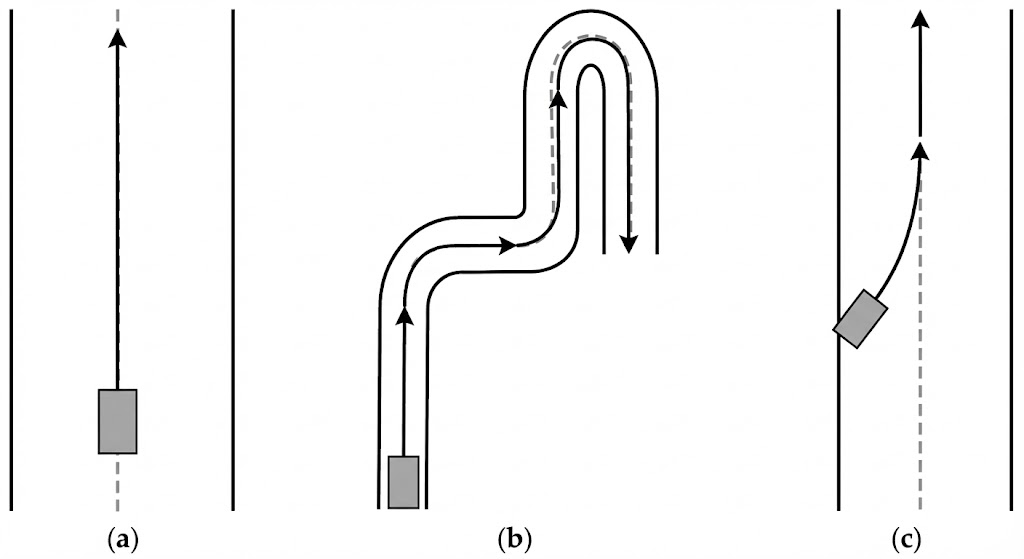
\includegraphics[width=1\linewidth]{figure_Eval_Scenarios.png}
    \caption{Schematic representation of the three experimental track configurations. (a) Scenario 1 tests straight-line stability on a straightforward path. (b) Scenario 2 evaluates the system's ability to handle sharp curvatures using 90-degree turns and a U-turn. (c) Scenario 3 tests generalization capability by initializing the robot with an offset position and misaligned heading, requiring it to recover to the path center.}
    \label{fig:testing_scenarios}
\end{figure}
\subsection{Performance Metrics}

To objectively quantify the navigation performance of the end-to-end controller, the study will utilize four primary metrics derived from the ground truth data captured by the overhead tracking system. The fundamental measure of tracking accuracy will be the Cross-Track Error (CTE). This is defined as the perpendicular distance between the robot's geometric center and the nearest point on the digital reference path at any given time step $t$. To provide a summary statistic for the entire run, the study will calculate the Root Mean Square Error (RMSE) of these deviations. A lower RMSE would indicate a tighter adherence to the reference path.
\begin{figure}[!ht]
    \centering
    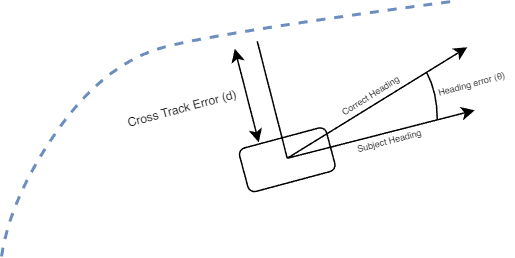
\includegraphics[width=0.8\linewidth]{images/figure_track_error.png}
    \caption{Visual Representation of Cross Track Error ($d$) and Heading Error ($\theta$).}
    \label{fig:cte_heading_error}
\end{figure}

Complementing the position error is the Heading Error, which evaluates the robot's orientation accuracy. This metric measures the angular difference between the robot's current yaw angle ($\theta_{robot}$) and the tangent angle of the path ($\theta_{path}$) at the nearest point. Monitoring heading error is critical for predictive analysis, as high angular deviations often precede a complete departure from the lane. Finally, the overall reliability of the system will be measured by the \textbf{Success Rate}, a qualitative metric calculated as the percentage of total attempts where the robot completed the entire course without any part of its chassis crossing the lane boundaries.